\section{SmartElement}

SmartElement är ett back-endsystem som sköter filtrering av innehåll på basis av information som samlas in om besökare på en webbsida. Upprätthållaren av en webbsida kan genom att integrera SmartElements JavaScript-tag i sin sida låta back-end systemet fylla i specificerade element med anpassat innehåll.

Systemet är i sig bara en motor för identifikation av användare och filtrering av innehåll. Det enda gränssnitt som SmartElement har är ett \gls{json}-gränssnitt genom vilket ett separat grafiskt gränssnitt tillåter användare att konfigurera sitt innehåll.

\subsection{Aktörer}

\begin{figure}[h!]
\centering
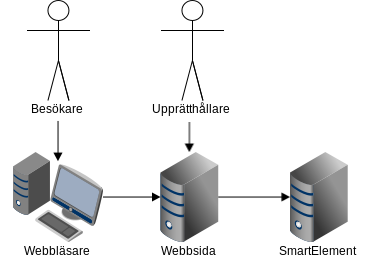
\includegraphics[width=150mm]{assets/images/smeleactors.png}
\caption{Aktörer}
\label{actors}
\end{figure}

Genom detta arbete används några aktörer för att förklara sammanhanget kring SmartElement. Närmast handlar det om besökaren, besökarens webbläsare, en webbsida, webbsidans upprätthållare samt SmartElement systemet.

Besökaren är den person som med sin webbläsare beöker webbsidan. Upprätthållaren är den person som upprätthåller en webbsida, på vilken denne installerat SmartElement-tagen. Med SmartElement ämnas, om ej annat nämns, back-endsystemet av SmartElement.

\subsection{Beståndsdelar}

\begin{figure}[h!]
\centering
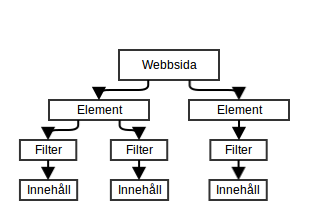
\includegraphics[width=120mm]{assets/images/smelementdatamodelabstract.png}
\caption{Exempel på en hierarki i SmartElement}
\label{abstractstructure}
\end{figure}

SmartElement bygger på några grundläggande koncept; webbsidor, element, filter och innehåll. Med dessa fyra byggstenar konfigureras objekt, visualiserat i figur \ref{abstractstructure}, som back-end systemet använder för att filtrera och leverera innehåll.

\subsubsection{Webbsidan}

Webbsidan är det högsta elementet i hierarkin som SmartElement handskas med. Det representerar en hel webbplats, under vilken man kan definiera element med innehåll. Varje sida har ett unikt identifikationsnummer som används för att ladda SmartElement-tagen.

\subsubsection{Element}

Elementen är hållare för den data som returneras från back-end systemet, de knyter innehållet till webbsidan. Elementet har i sig flere innehåll och filter. Filtren används för att välja ut det innehåll som skall visas i elementet. Element har en inom webbsidan unik kod som används för att specificera vilka element som behöver processeras när man anropar back-end systemet.

\subsubsection{Filter}

Filter består i SmartElement av flera olika regler som ställer en fråga om besökaren och har en länk till ett innehåll, vilket visas om filtret matchar. För att ett filter skall matcha krävs det att besökaren passar alla regler i filtret. För att hantera fall var två eller flera filter passar för en besökare, har filter en prioritets-ordning inom elementet som användaren själv kan definiera.

\subsubsection{Innehåll}

Innehåll är den konkreta data som levereras för ett element efter att ett filter valts som vinnare. Innehållet kan bestå av text, HTML-kod eller \gls{json}-data, hurudan som helst data som kan sparas som en textsträng. Det är upp till användaren att definiera vad för data som sparas.

\subsection{Funktion}

SmartElement har två huvudsakliga funktionsområden. Konfiguration av systemet genom API-gränssnittet samt hantering av sidvisningar och filtrering av innehåll genom innehålls-gränssnittet.

\subsubsection{Konfiguration}

\begin{figure}[h!]
\centering
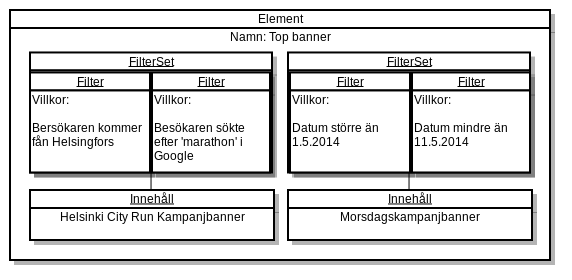
\includegraphics[width=150mm]{assets/images/smelementelement.png}
\caption{Exempel på en elementkonfiguration}
\label{smelementelement}
\end{figure}

För att SmartElement skall kunna leverera innehåll, måste användaren konfigurera sidan och dess element på förhand. Processen består av att registrera element under sidobjektet, skapa innehåll samt att konfigurera filter genom att kombinera regler om vilka användare innehållet passar för.

I praktiken sker all konfiguration av systemet, då det är i produktion, genom ett \gls{json} gränssnitt. En klient kopplar upp sig, autentiserar sig med en nyckel och kan sedan göra förfrågningar mot gränssnittet.

Konfigurationsprocessen börjar med att registrera en webbsida i systemet. En användare kan ha flera olika sidor registrerade i systemet, så gränssnittet jobbar alltid under en utvald webbsida.

Under webbsidan kan användaren registrera de element för vilka innehållet skall anpassas. Elementen är i grund och botten bara nycklar som används för att representera objekt som kan se ut på olika sätt (ha olika innehåll) beroende på de filter som associeras med dem.

Efter konfiguration av element konfigureras ett eller flera innehåll under dessa. I samband med innehållen lägger användaren till filter i innehållets filter-set. Alla filter som registreras måste passa för att ett innehåll skall visas. Genom dessa filterkombinationer kan avancerade villkor implementeras.

\subsubsection{Sidvisning}

\begin{figure}[h!]
\centering
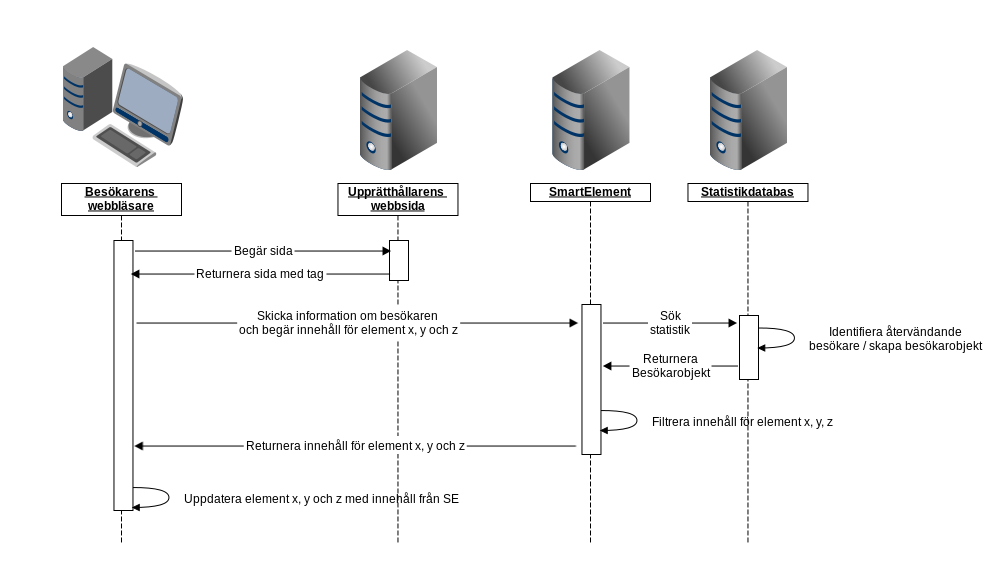
\includegraphics[width=150mm]{assets/images/smelementactivity.png}
\caption{Processen vid en sidvisning}
\label{pageviewprocess}
\end{figure}

Figur \ref{pageviewprocess} representerar kommunikationen vid en sidvisning. När en användares webbsida laddas, inkluderar den en JavaScript fil som innehåller SmartElements tag. Efter att sidan laddats klar körs tagen, som samlar ihop information om besökaren, samt eventuell extra data som användaren specificerat i tagen, och skickar informationen till back-enden. På back-enden kombineras informationen från tagen med eventuell statistikdata från en statistikdatabas för att skapa ett besökarobjekt.

Backenden tar emot besökarobjektet och söker upp sidan som motsvarar det id som skickats. Efter att en sida har hittats går back-enden igenom de element som tagen begär innehåll för och filtrerar deras innehåll på basis av datan i besökarobjektet. Allt innehåll kompileras till en lista med element-id länkat till innehåll och skickas tillbaka till besökarens webbläsare.

Om användaren inte valt att ändra på beteendet av tagen så anropar back-enden på tagen för att fylla elementen med den data som returnerats.
